\hypertarget{st__init_8c}{
\section{st\_\-init.c File Reference}
\label{st__init_8c}\index{st_init.c@{st\_\-init.c}}
}


\subsection{Detailed Description}
\begin{Desc}
\item[For internal use only.]
This file contains the implementation of the \hyperlink{group__dbprim__smat_ga10}{st\_\-init()} function, used to dynamically initialize a sparse matrix table.\end{Desc}


Definition in file \hyperlink{st__init_8c-source}{st\_\-init.c}.

{\tt \#include \char`\"{}dbprim.h\char`\"{}}\par
{\tt \#include \char`\"{}dbprim\_\-int.h\char`\"{}}\par


Include dependency graph for st\_\-init.c:\begin{figure}[H]
\begin{center}
\leavevmode
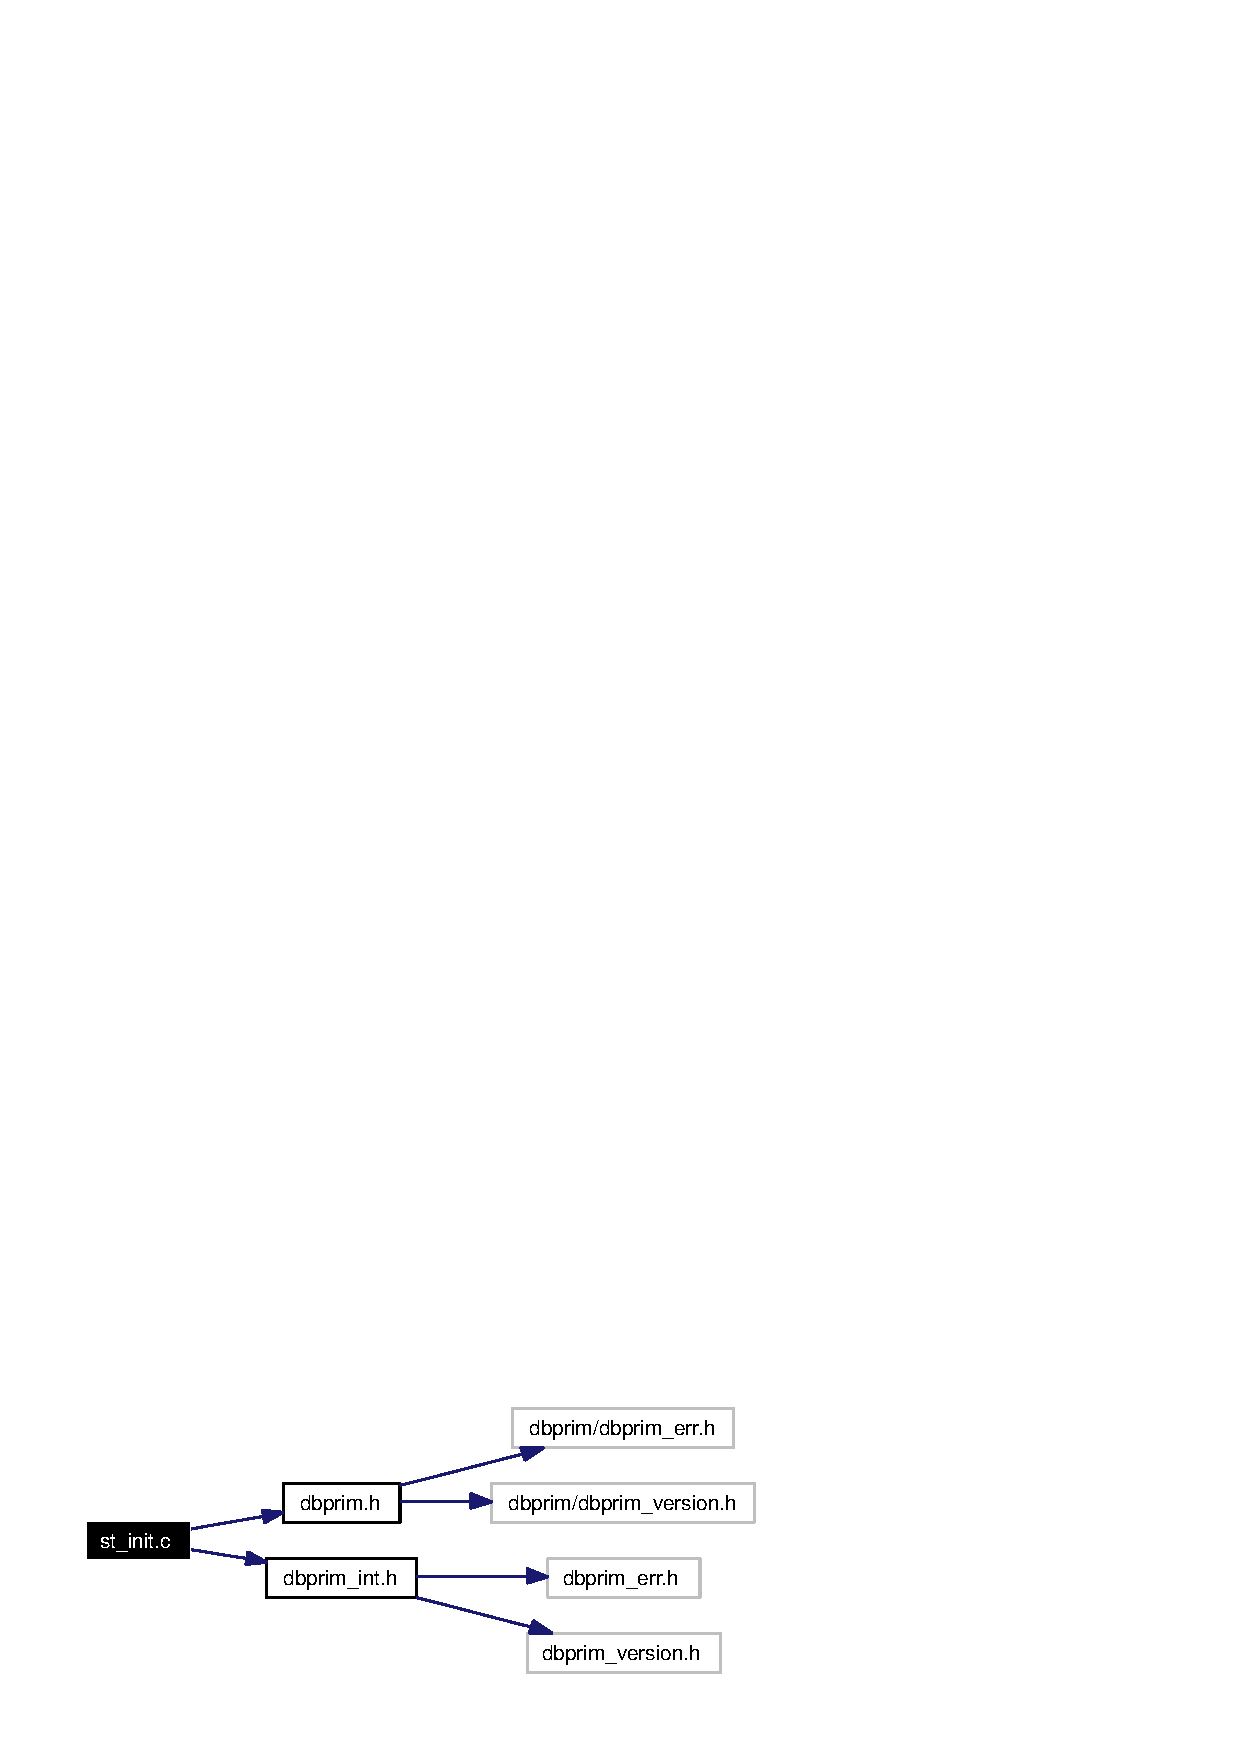
\includegraphics[width=183pt]{st__init_8c__incl}
\end{center}
\end{figure}
\subsection*{Functions}
\begin{CompactItemize}
\item 
unsigned long \hyperlink{group__dbprim__smat_ga10}{st\_\-init} (\hyperlink{struct__smat__table__s}{smat\_\-table\_\-t} $\ast$table, unsigned long flags, \hyperlink{group__dbprim__smat_ga3}{smat\_\-resize\_\-t} resize, void $\ast$extra, unsigned long init\_\-mod)
\begin{CompactList}\small\item\em Dynamically initialize a sparse matrix table. \item\end{CompactList}\end{CompactItemize}
